\chapter{Conclusion}
\setlength{\epigraphwidth}{.45\textwidth}
\epigraph{All models are wrong, but some are useful.}{George E. P. Box}

The mapping for a single position using all beams is displayed in figure
\ref{fig:truth_map}. This figure also contains a thin green line representing
the ground truth for the box-like environment used as input to the simulator.

\begin{figure}[ht]
    \centering
    \subfloat[ Plane
    $x=0$]{{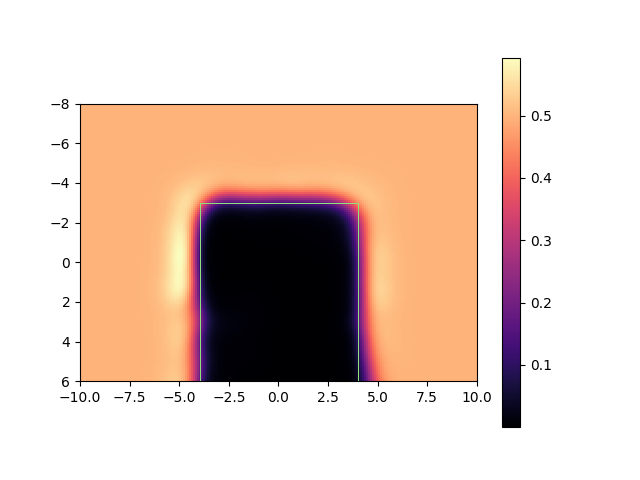
\includegraphics[width=75mm,trim={0 14mm 0
    10mm},clip]{Chap5/fig/wall_one_full_x_0}}}%
    \hfill \subfloat[ Plane
    $z=-1$]{{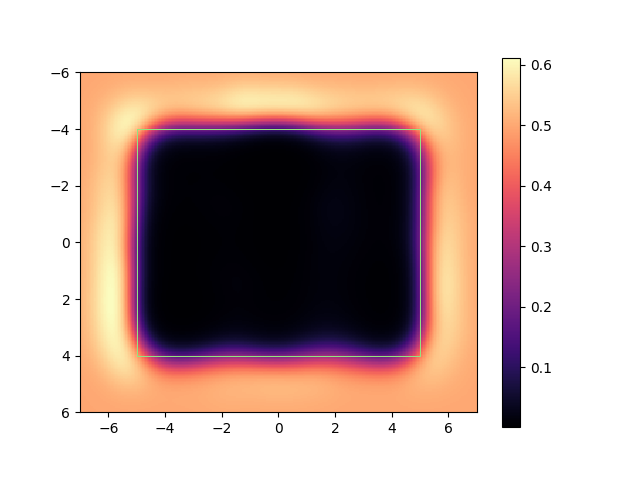
\includegraphics[width=75mm,trim={0 14mm 0
    10mm},clip]{Chap5/fig/wall_one_full_z_-1}}}%
    \caption{Mapping using only 1 position and 3 sonar orientations with
    ground truth as green lines.}%
    \label{fig:truth_map}%
\end{figure}

Qualitatively, the empty region is almost perfectly reconstructed, with corners
smoothed out. However the walls themselves are over a region of probability
$\approx35\%$. This low probability value can be explained as consequence of
having a highly reliable information about emptyness in contrast with a
diffuse measurement of occupied regions. Such a difference, together with a smooth kernel
space may create a slow change between the regions, biased towards empty space.
The smoothed corners may also be partially caused by the choice of
kernel and its approximation.

Nevertheless, the Hibert Maps applied to the underwater problem manifest a
depiction of the environment clear enough for humans to read and still have a
promising result for localization. The maximum error between the ground truth
and the half probability region was about $45$cm (Fig.\ref{fig:halfprob})


\begin{figure}[h]
	\centering
	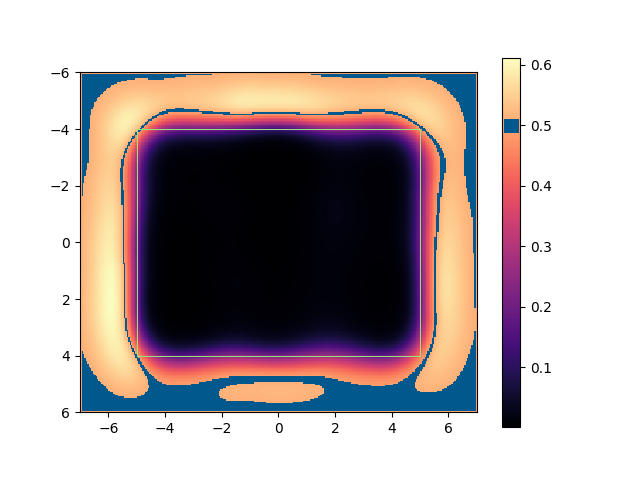
\includegraphics[width=0.8\textwidth]{Chap5/fig/wall_one_full_z_-1_change}
	\caption{Blue region is the half probability region and green lines represent
	ground truth.}
	\label{fig:halfprob}
\end{figure}

\section{Future Works}

On the simulation side, resonable next steps include implementing a more complex
BDRF to emulate more realistic materials, although that depends on measurements
which creates an extra difficulty. Also experimentation with Metropolis
Transport similar methods that could improve less sharp shadows and caustics
depiction.

The mapping with Hilbert maps is a parametric method, thus automatic selection
is a simple incremental change, which may also include other feature
approximations. A post processing step could be also envisioned, an optimization
step, with a forward sonar model (simulation), to generate sharper corners and
retrieve information about the surroundings, similar to elevation maps optimization (section
\ref{ss:mapsoffeatures}).
